\documentclass[PICOReport.tex]{subfiles}

\begin{document}

\subsubsection{Gravitational Waves and Inflation}
\label{sec:inflation}

%\paragraph{Targets}
\noindent$\bullet$ {\bf Targets} \hspace{0.1in} 

According to Einstein's theory of general relativity, the density perturbations responsible for the observed CMB anisotropy must have been created long before the \ac{CMB} was released, and even before the Universe became filled with a hot and dense plasma of fundamental particles. Understanding the mechanism generating these perturbations, which evolved to fill the Universe with structures, is one of the most important open questions in cosmology. In addition to density perturbations, this mechanism may have also produced gravitational waves that would have left a $B$-mode polarization signature in the CMB~\cite{seljak97,kamionkowski97a}.  Any detection of primordial $B$-mode polarization by PICO will constitute evidence for gravitational waves from the same primordial period that created the density perturbations and will open a new window onto this early epoch. Because the dynamics of gravitational waves is essentially unaffected by the plasma, they would be a pristine relic from the earliest moments of our Universe, and their properties would shed light on the mechanism that created the primordial perturbations. 

Inflation, a period of nearly exponential expansion of the early Universe~\cite{Guth:1980zm,Linde:1981mu,Albrecht:1982wi,Starobinsky:1980te}, is the leading paradigm explaining the origin of the primordial density perturbations~\cite{Mukhanov:1981xt,Guth:1982ec,Hawking:1982cz,Starobinsky:1982ee,Bardeen:1983qw}. It predicts a nearly scale-invariant spectrum of primordial gravitational waves originating from quantum fluctuations~\cite{Starobinsky:1979ty}. Measurements of the \ac{CMB} are the only foreseeable way to detect these gravitational waves.
%\sout{In this sense, a detection of primordial $B$-modes would be the first observation of a phenomenon associated with quantum gravity~\cite{Krauss:2013pha}.} \comor{moved} 

\begin{figure}[!thb]
\centering
\vspace{-0.05in}
\hspace{-0.15in}
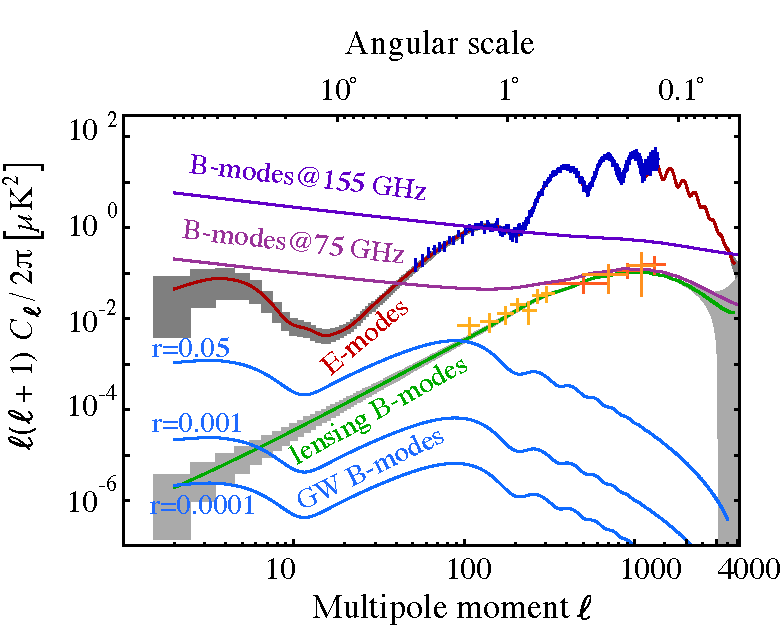
\includegraphics[width=3in]{images/cmb_powspec_PICOv4p1_v2.pdf}
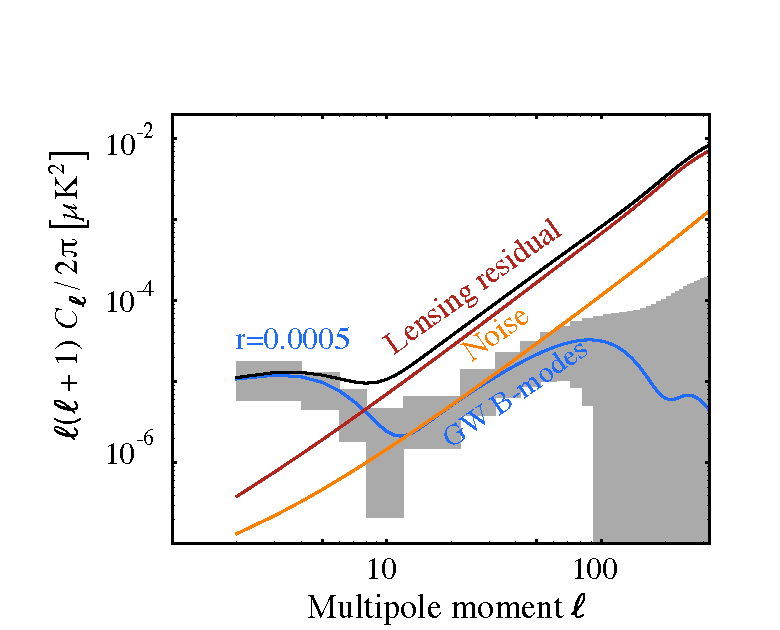
\includegraphics[width=3in]{images/cmbbb_powspec_PICOv4p1_v4.pdf}
\vspace{-0.1in}
\caption{\captiontext With PICO's baseline configuration we will measure the $EE$ (left, red) and lensing $BB$ (green) angular power spectra with high precision (grey). PICO's goal is to detect $r= 5\times 10^{-4}\, (5\sigma)$ (right, grey). This forecast includes PICO's 80\% delensing (red) and foreground separation. The baseline noise level (right, orange) allows detection of even lower levels; we expect foreground separation to limit performance.  As an example we show the total $BB$ spectra on the cleanest $60\%$ of the sky at 75 and 155~GHz (left, purple). The foregrounds largely dominate the cosmological signals. Also shown are measurements of lensing from current experiments (left, orange)~\citep{PB_BB, keisler2015, actpol_lensing_BB, Array:2015xqh}, \planck 's $EE$ measurements (left, dark blue)~\citep{Planck2018_I}, and the $BB$ spectrum produced by an inflationary gravity wave (GW) signal with different values of $r$ (cyan). 
\label{fig:clbb} }
\vspace{-0.05in}
\end{figure}

The strength of the signal, quantified by the tensor-to-scalar ratio $r$, is a direct measure of the expansion rate of the Universe during inflation. Together with the Friedmann equation, it reveals one of the most important characteristics of inflation: its energy scale.\footnote{In some models of inflation the one-to-one correspondence between $r$ and the energy scale of inflation does not hold because there are additional sources of gravitational waves~\cite{Namba:2015gja}. However, in these models the signal is highly non-Gaussian and could be distinguished from models without such sources, for which the signal is Gaussian.}  A detection of $r$  ``would be a watershed discovery'', a quote from the 2010 decadal panel report~\citep{blandford2010}. The combination of data from \planck\ and the BICEP/Keck Array give the strongest constraint to date, $r<0.06\,\, (95\%)$~\citep{bicep_keck2018}. Next decade S3 efforts strive to reach $\sigma(r)=2 \times10^{-3}$~\citep{SOscience, biceparray}.

PICO will detect primordial gravitational waves if inflation occurred at an energy scale of at least $5\times 10^{15}\,\rm{GeV}$, or equivalently $r= 5\times 10^{-4} \, (5\sigma)$ (SO1 in Table~\ref{tab:STM} and Fig.~\ref{fig:clbb}).  A detection will have profound implications for fundamental physics. It will provide evidence for a new energy scale tantalizingly close to the energy scale associated with grand unified theories, probe physics at energies far beyond the reach of terrestrial colliders, and be the first observation of a phenomenon associated with quantum gravity~\cite{Krauss:2013pha}.

%PICO's goal is to detect primordial gravitational waves if inflation occurred at an energy scale of at least $5\times 10^{15}\,\rm{GeV}$, or equivalently $r= 5\times 10^{-4} \, (5\sigma)$ (SO1 in Table~\ref{tab:STM} and Fig.~\ref{fig:clbb}).  A detection will have profound implications for fundamental physics. It will provide evidence for a new energy scale tantalizingly close to the energy scale associated with grand unified theories, probe physics at energies far beyond the reach of terrestrial colliders, and be the first observation of a phenomenon associated with quantum gravity~\cite{Krauss:2013pha}.

There are only two classes of slow-roll inflation in agreement with current data that naturally explain the observed value of the spectral index of primordial fluctuations $n_{\rm s}$~\cite{Aghanim:2018eyx}. The first class is characterized by potentials of the form $V(\phi)\propto\phi^p$. This class includes many of the simplest models of inflation, some of which have already been strongly disfavored by existing observations. Select models in this class are shown as blue lines in Fig.~\ref{fig:nsr}. When the constraints on $n_{\rm s}$ tighten by about a factor of two with the central value unchanged, and the upper limit on $r$ improves by an order of magnitude, this class would be ruled out. 

The second class is characterized by potentials that approach a constant as a function of field value, either like a power law or exponentially. Two representative examples in this class are shown as the green and gray bands in Fig.~\ref{fig:nsr}. This class also includes $R^2$ inflation, which predicts a tensor-to-scalar ratio of $r\sim 0.004$. All models in this class, with a characteristic scale in the potential that is larger than the Planck scale, predict a tensor-to-scalar ratio of $r\gtrsim 0.001$. PICO will definitively exclude these models, or will detect gravitational waves; either result will be achieved with more than $5\sigma$ confidence. 
While many microphysical models in this second class possess a characteristic scale that is super-Planckian, some have a somewhat smaller scale. One example is the Goncharov-Linde model, which predicts a tensor-to-scalar ratio of $r\sim 4\times 10^{-4}$~\cite{Goncharov:1983mw}, still within detection reach by PICO~(Fig.~\ref{fig:nsr}). There are models with smaller values that are out of reach.  

This much is clear: if the PICO required threshold is passed without a detection, most textbook models of inflation will be ruled out and the data would force a significant change in our understanding of the primordial universe.

%Distinguishing between models with sub- and super-Planckian characteristic scales would provide much needed guidance to discriminate between classes of ideas for the physics of the earliest moments of our Universe.

%While many microphysical models in this second class possess a characteristic scale that is super-Planckian, some have a somewhat smaller scale. One example is the Goncharov-Linde model, which predicts a tensor-to-scalar ratio of $r\sim 4\times 10^{-4}$~\cite{Goncharov:1983mw}, still within detection reach by PICO~(Fig.~\ref{fig:nsr}). There are models with significantly smaller values that are out of reach.  

%Distinguishing between models with sub- and super-Planckian characteristic scales would provide much needed guidance to discriminate between classes of ideas for the physics of the earliest moments of our Universe.


\begin{figure}[!thb]
\parbox{4.5in}{\centerline{
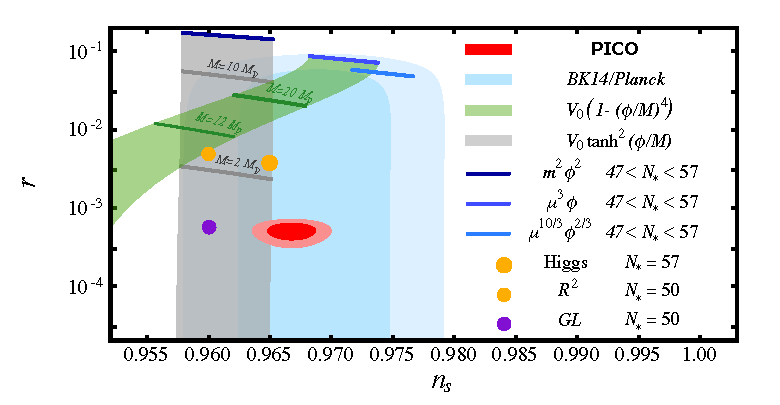
\includegraphics[width=4.5in]{images/nsrlabeledrp0005_PICOv2.pdf} } }
\parbox{1.8in}{
\caption{\captiontext  Current $1\sigma$ and 2$\sigma$ limits on $r$ and $n_{\rm s}$ (cyan) and forecasted constraints for a fiducial model with $r = 0.0005$ for PICO, together with predictions for selected models of inflation. Characteristic super-Planckian scales in the potentials are marked with darker lines. GL is the Goncharev-Linde model (see text). }
\label{fig:nsr}}
\vspace{-0.1in}
\end{figure}

%\paragraph{Observational Considerations}
\noindent$\bullet$ {\bf Observational Considerations} \hspace{0.1in} 
The $BB$ angular power spectrum measured by PICO will have contributions from Galactic sources of emission and `lensing' $B$-modes, created by gravitational lensing of $E$-modes as the CMB photons traverse the gravitational potentials throughout the Universe (Fig.~\ref{fig:clbb} and \S\,\ref{sec:gravitationallensing}). In case of an $r$ detection, there will be two additional features due to the inflationary signal. One is the `recombination peak' at $\ell = 80$ and the other is the `reionization peak' at multipoles of $\ell\lesssim 10$. PICO's strong constraints on $r$ derive from using all available $\ell$ modes.

The Galactic signals act as foregrounds, and uncertainty in the characterization of these foregrounds already limits our ability to constrain $r$. 
%PICO's goal for reaching $\sigma(r) = 1\times10^{-4}$ is driven by estimates of the efficacy of foreground separation, not noise.  
An analytic performance forecast accounting for PICO's statistical noise level and a foreground model that has polarized emission from two components of dust, synchrotron radiation, and correlations between synchrotron and dust emission, gives $\sigma(r) = 2\times10^{-5}$, five times lower than our baseline requirement. This margin allows for degradation in foreground removal through inclusion of physical effects known to exist but not captured in the analytic forecasts. These effects are included in end-to-end, map-based simulations, which indicate that PICO will achieve its requirement; see Section~\ref{sec:signal_separation}. 
%\comor{say more?}

%Our goal is set based on end-to-end, map-based simulations, which include physical effects known to exist but not captured in the analytic forecasts; see Section~\ref{sec:signal_separation}.   
%such as spatial variation of dust temperatures, dust-to-gas ratio, dust composition, which lead to spatial variation of the spectral dependence, are expected to weaken the constraints. In Section~\ref{sec:foregrounds} we discussed PICO's capability to separate foregrounds in more detail. 

%The Galactic signals act as foregrounds and uncertainty in the characterization of these foregrounds already limits our ability to constrain r.  End-to-end map-based simulations using PICO?s statistical noise level and a foreground model that has polarized emission from two components of dust, synchrotron radiation, and correlations between synchrotron and dust emission, gives s(r) = 2?10?5, five times lower than our requirement (s(r)=1?10?4). This margin allows for physical effects known to exist but not yet captured in the analytic forecasts; see Section 2.5.

When the tensor-to-scalar ratio $r \simeq 0.01$, the $BB$ lensing and inflation spectra are comparable in magnitude at the recombination peak $(\ell = 80)$. For lower levels of $r$, the lensing $B$-mode dominates, but the $B$-mode maps can be `delensed' if the polarization maps are measured with few-arcmin resolution and sufficient depth~\citep{2004PhRvD..69d3005S,2012JCAP...06..014S}. Forecasts for PICO show that at least 73\% of the lensing $B$-mode power can be removed for the baseline configuration, after accounting for conservative Galactic foreground separation. As much as 84\% will be removed for the CBE and for milder foreground contamination. For measuring the recombination peak, delensing is essential in order to reach PICO's limits on $r$, and this was a driver in choosing the resolution of the instrument. 
% PICO will be relying on its own data to conduct delensing, thus avoiding increased noise from the need to cross-calibrate experiments, identify common observing areas on the sky, not having frequency-band coverage at the appropriate resolution to remove foregrounds, or from other systematic uncertainties.

For the levels of $r$ targeted by PICO, the $BB$ reionization signal $(\ell < 10)$ has a somewhat higher level than the lensing spectrum, but the map-level foregrounds at this angular scale are at least two orders of magnitude brighter.  There are currently no $BB$ measurements at these scales, and no S3 experiments plan to measure $B$-modes that reach to $\sigma(r) < 0.006$ in the lowest multipoles~\citep{class,piper}. PICO's instrument temporal stability, absence of atmospheric noise, full-sky coverage, and unmatched capability to characterize and separate foregrounds make it the most suitable instrument to measure these lowest multipoles (\S\,\ref{sec:signal_separation}).

If an inflationary $B$-mode signal is detected, it is important to characterize its entire $\ell$ dependence in the predicted reionization and  recombination peaks, in order to confirm -- rather than assume -- its expected dependence on angular scale.  Furthermore, the PICO full-sky coverage will enable detection of the recombination peak in several independent patches of the sky, giving an important systematic cross-check. 

\noindent$\bullet$ {\bf Scalar Spectral Index and Non-Gaussianity} \hspace{0.1in} Models of the early Universe differ not only in their predictions for $r$ and the scalar spectral index $n_{\rm s}$, but also for the scale-dependence of $n_{\rm s}$, a parameter commonly called ``the running of $n_{\rm s}$'' and labeled $n_{\rm run}$. PICO will improve $n_{\rm s}$ and $n_{\rm run}$ constraints by a factor of three relative to \planck\ to achieve $\sigma(n_{\rm s})=0.0015$ and $\sigma(n_{\rm run})=0.002$. For many models of inflation, how reheating occurred is unknown, and this translates to different predictions for $n_{\rm s}$ and $n_{\rm run}$~\citep{planck2018_inflation}. PICO's precision is sufficient to distinguish between different possible reheating scenarios at $>3\sigma$ (SO2). 

The simplest models of inflation, in which there is a single inflaton field, predict primordial fluctuations that are very nearly Gaussian with $|f^{\rm local}_{\rm NL}| <1$, where $f^{\rm local}_{\rm NL}$ is a parameter quantifying the level of local non-Gaussianity~\citep{planck2015_17}. A detection of $|f^{\rm local}_{\rm NL}| >1$ points exclusively to models of inflation with multiple fields (Fig.~\ref{fig:fnlconstraint}). 
%, making $\sigma (f^{\rm local}_{\rm NL}) < 1$ a compelling target. 
\planck\ gives a constraint of $f^{\rm local}_{\rm NL} = 0.8 \pm 5 \, (1\sigma)$~\citep{planck2015_17}, and further measurements of the \ac{CMB} alone cannot improve on this constraint by more than a factor of 2--3. However, correlating large-scale structure tracers that have different clustering bias factors can enhance the signature of non-Gaussianity~\citep{2009PhRvL.102b1302S,2018PhRvD..97l3540S,2008PhRvD..77l3514D}. Fig.~\ref{fig:fnlconstraint} shows expected constraints from correlations between the PICO lensing potential maps (\S~\ref{sec:gravitationallensing}) and LSST galaxies. For $f^{\rm local}_{\rm NL}=2$, $3\sigma$ evidence will be reached if large angular scale ($L\ge 8$)\footnote{$L$ refers to multipoles in galaxy clustering fields and in CMB lensing~(\S~\ref{sec:gravitationallensing}), in contrast to the use of $\ell$  for the CMB itself. \label{foot:L}} auto- and cross-correlation spectra can be used. If LSST's auto-correlation can only be used on smaller angular scales $L\ge 20$, the $3\sigma$ evidence weakens to $2\sigma$. 
%Specifically, using data spanning angular scales with $L>6$ a compelling constraint of $|f_{NL}|<1\, (2\sigma)$ will be reached. 

\begin{figure}[h]
\hspace{-0.in}
\parbox{3.0in}{{
% 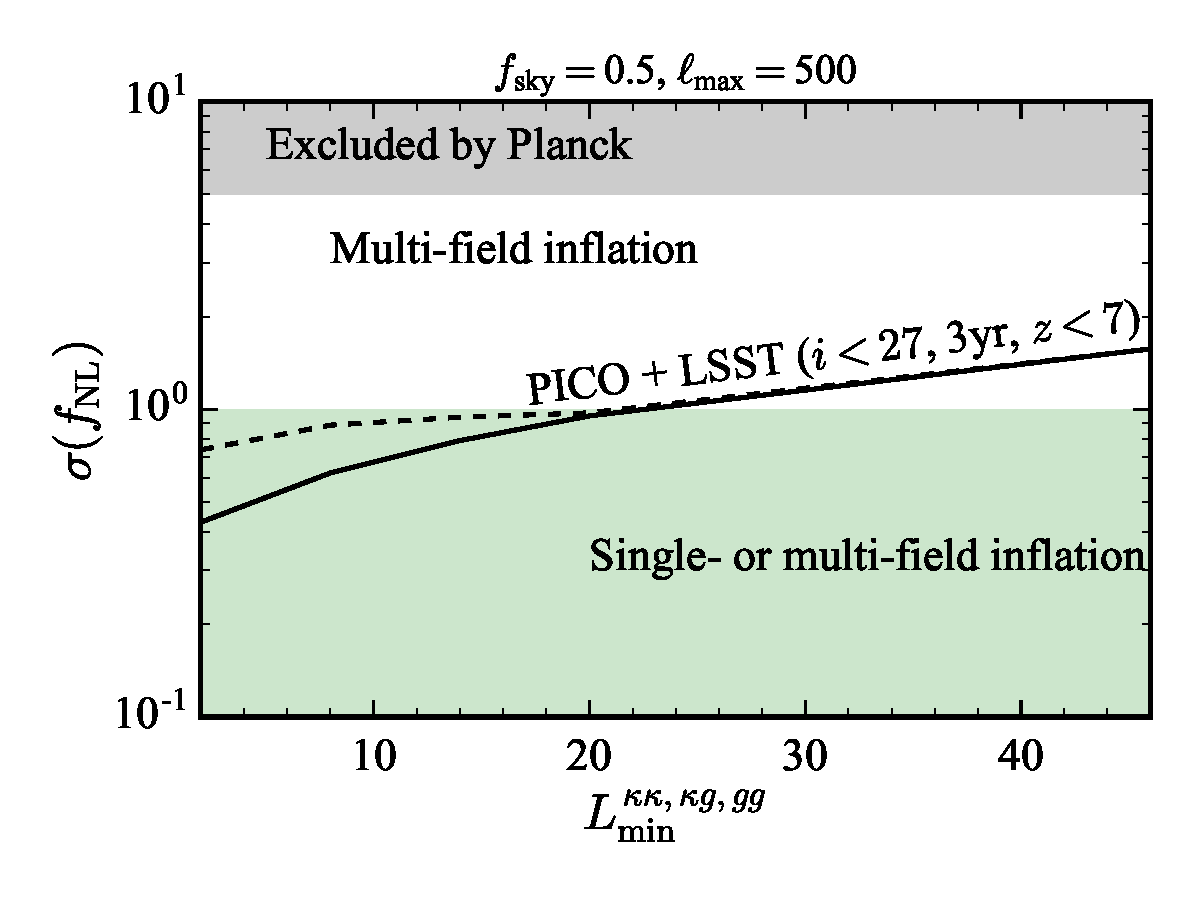
\includegraphics[width=2.95in]{images/PICO_fnl_lmin_PICOv4.1b_deproj0_SENS0.pdf} } }  % pre Dec. 20th version
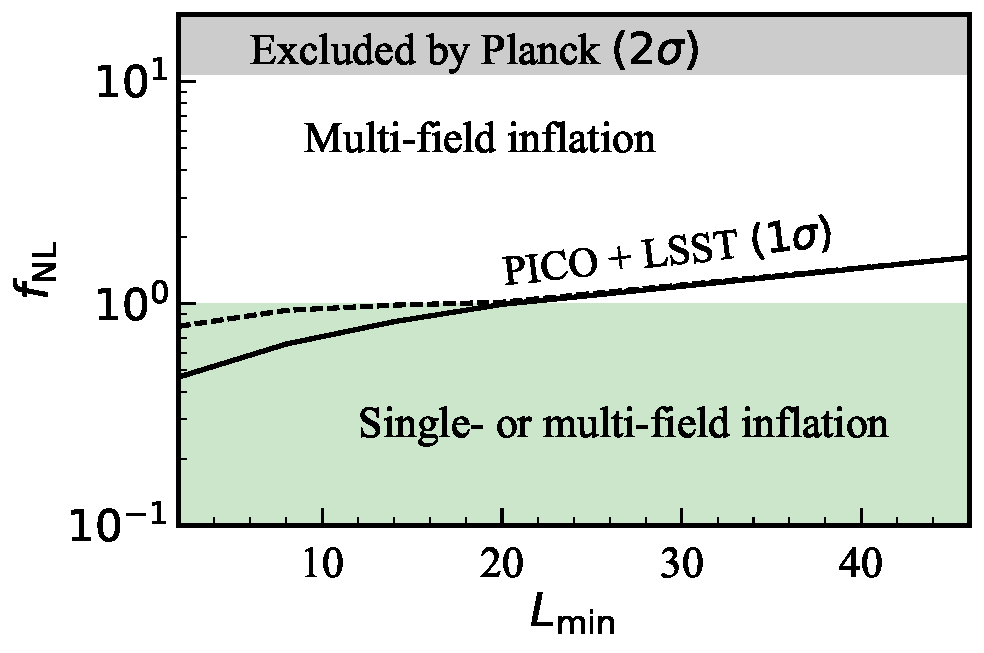
\includegraphics[width=2.95in]{images/PICO_fnl_lmin_PICOv4.1b_deproj0_SENS0_LSST10yrGoldWithDropouts.pdf} } }   % new version, LSST gold, 10year
\hspace{0.in}
\parbox{3.4in}{
\caption{\captiontext
Cross-correlating PICO's lensing potential map with LSST galaxies will allow detecting or excluding  $f^{\rm local}_{\rm NL}=2$ with $3\sigma$ evidence  if the data can be used at  angular scales $L \ge 8$ (solid black). A detection above $|f^{\rm local}_{\rm NL}| =1$ indicates that inflation is driven by multiple fields; single-field inflation has $|f^{\rm local}_{\rm NL}|<1$ (green region). The \planck\ constraint is $f^{\rm local}_{\rm NL} < 10.8\, (2\sigma)$. The cross-correlations will allow excluding or detecting $f^{\rm local}_{\rm NL}=2\, (2\sigma)$ if LSST data are used only for $L\ge 20$ (dash). Fig.~\ref{fig:sigma8} gives the assumptions used here for the LSST data. 
\label{fig:fnlconstraint}
} }
\vspace{-0.1in}
\end{figure}

%\comor{One can use correlations between large-scale structure tracers with different clustering bias factors and measure the relative difference between their clustering power spectra to effectively cancel cosmic variance~\citep{2009PhRvL.102b1302S,2018PhRvD..97l3540S}; this can constrain physics that affects the biasing of objects on large scales, such as primordial local non-Gaussianity~\citep{2008PhRvD..77l3514D}.  In Fig.~\ref{fig:fnlconstraint} we show the expected constraints for the CMB lensing field as reconstructed with PICO, in cross-correlation with  three years of the LSST survey. It can be seen that depending on the minimal multipole that can be used in the cross correlation, which is uncertain in both LSST and the PICO lensing map, the well-motivated theory target of $\sigma (f_\mathrm{NL}) \simeq 1$ \citep{2014arXiv1412.4671A} can be within reach. Values of $f_\mathrm{NL}$ at or above this level are a generic prediction of multi-field inflationary models.}


\subsubsection{Fundamental Particles: Light Relics, Dark Matter, and Neutrinos}
\label{sec:relics_neutrinos}

%%%%%%%%%%%%%%%%%%%%%%%%%
$\bullet$ {\bf Light Relics} \hspace{0.1in} In the inflationary paradigm, the Universe was reheated to temperatures of 
at least 10 MeV and perhaps as 
high as $10^{12}$ GeV.  At these high temperatures, even very weakly interacting or very massive particles, 
such as those arising in extensions of the Standard Model of particle physics, can be produced in large 
abundances~\cite{1979ARNPS..29..313S,Bolz:2000fu}.  As the Universe expands and cools,
the particles fall out of equilibrium, an event referred to as `decoupling,' and characterized by a decoupling temperature $T_{F}$.  The decoupling leaves observable signatures in the CMB power spectra. Through these effects the CMB is a sensitive probe of neutrino and other particles' properties.  

% sensitive probe of the fundamental particle content in the Universe
% large abundance, but not large enough to leave present day signatures? or they decay?
% don't like the words 'extensions of ...' suggests very unlikely things. 

One particularly compelling target is the effective number of light relic particle species $\Neff$. The canonical value with three neutrino families is $\Neff = 3.046$. Additional light particles contribute a change $\Delta \Neff$ that is a function only of the decoupling temperature and the spin of the particle~$g$. The magnitude of $\Delta\Neff$ is quite restricted, even for widely varying decoupling temperatures $T_{F}$. A range $ 0.027\,g \leq \ \Delta \Neff \leq 0.07\,g$ corresponds to a range in $T_{F}$ spanning decoupling during post-inflation reheating (0.027$g$) down to lower $T_{F}$ with decoupling occurring just prior to the QCD phase transition ($0.07g$).
%Additional light particles contribute a universal change to $\Neff$ that is a function only of the decoupling temperature and the effective degrees of freedom of the particle, $g$. Furthermore, the range of $\Delta\Neff$ is quite restricted, even for widely varying decoupling temperatures $T_{F}$ with the range $ 0.027\,g \leq \ \Delta \Neff \leq 0.07\,g$ corresponding to decoupling at higher temperatures during post-inflation reheating (0.027$g$) to lower temperatures shortly prior to the QCD phase transition ($0.07g$).

Information about $\Neff$ is gleaned primarily from the $TT,\, TE$, and $EE$ power spectra. For an experiment like PICO, which has sufficient resolution to reach a cosmic-variance-limited measurement\footnote{A measurement is cosmic-variance-limited when the measurement uncertainty is dominated by the statistics of observing the finite number of spherical harmonic decomposition modes available in our Universe.} of $EE$ up to $\ell =2300$, the two additional most important parameters for improving constraints are the fraction of sky observed, $f_{\rm sky}$, and the noise (Fig.~\ref{fig:Neff_future}, left). The PICO baseline will use data from 70\% of the sky to constrain $\Delta \Neff < 0.06 \, (95\%)$ (S04).\footnote{The CMB $EE$ and the Galactic foregrounds $EE$ and $BB$ spectra are comparable in level (Fig.~\ref{fig:clbb}). With 21 frequency bands PICO should be able to separate signals at the mild levels necessary for $EE$ over 70\% of the sky~(\S~\ref{sec:signal_separation}).} This constraint, which is a factor of 4.7 improvement relative to \planck~($\Delta \Neff < 0.28$, 95\%) and will not be matched by any currently funded effort, opens up a new range of temperatures in which to detect the signature of light relic species. If no new species are detected, then the lowest temperature $T_{F}$ at which any %particle with spin 
vector particle (spin 1) could have fallen out of equilibrium will move up by a factor of 400 (Fig.~\ref{fig:Neff_future}, right). 

\begin{figure}[t!]
\begin{center}
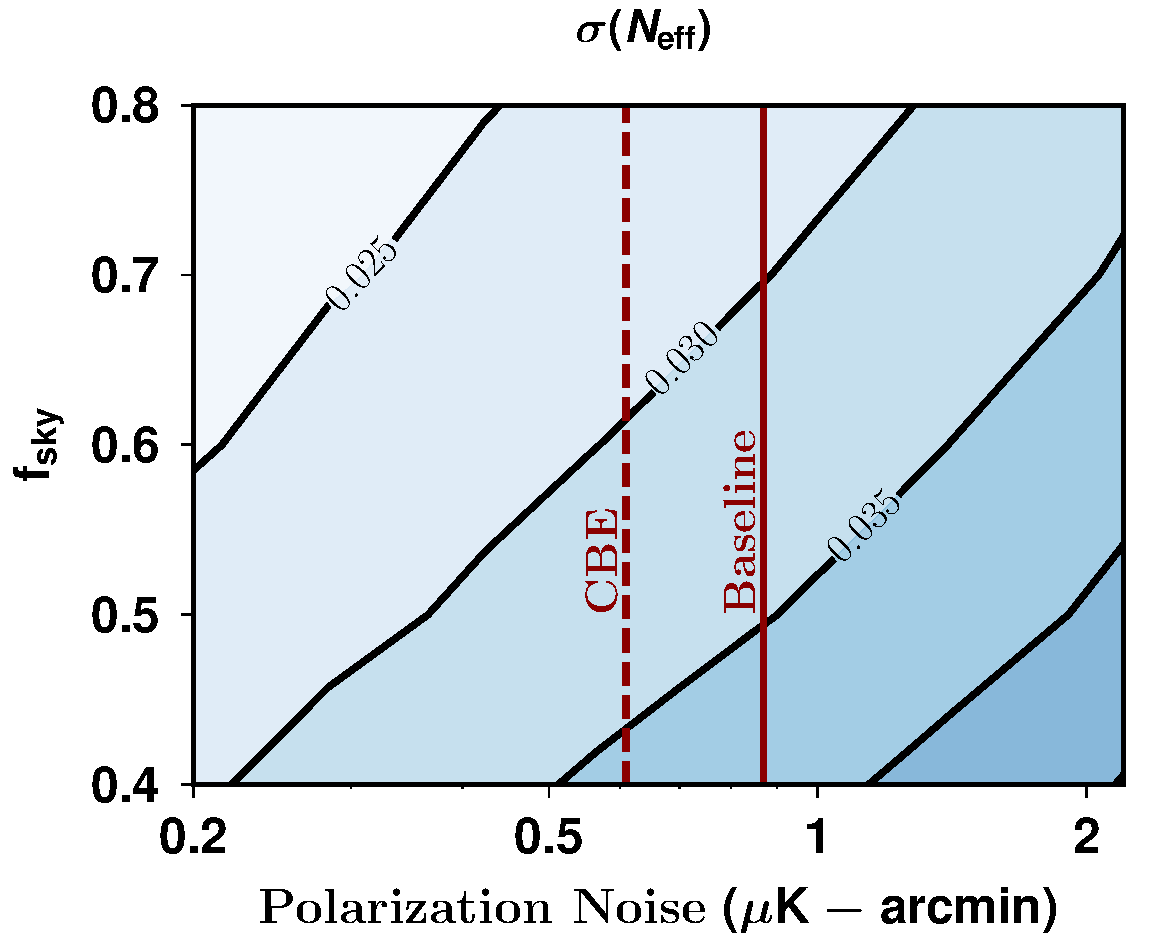
\includegraphics[width=0.45\textwidth]{images/Neff_final.pdf}
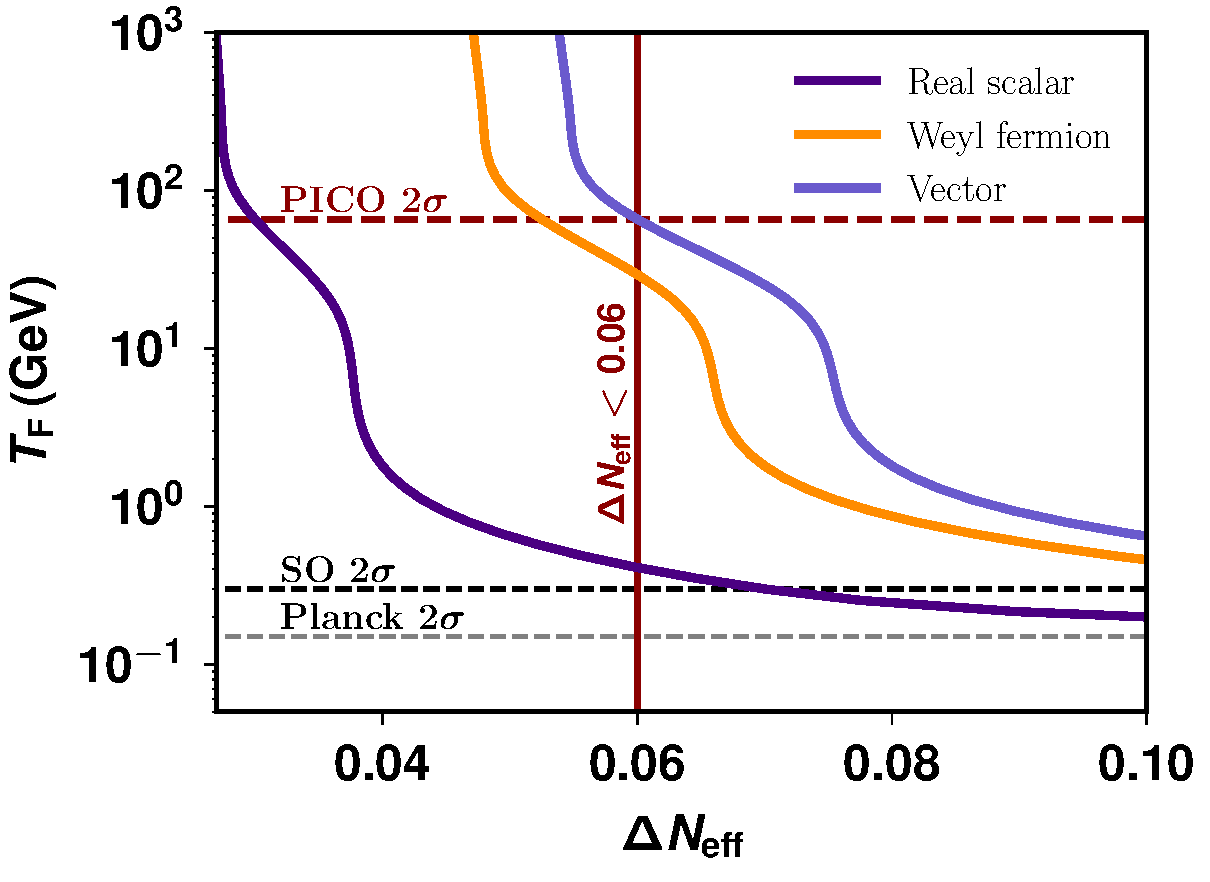
\includegraphics[width=0.47\textwidth]{images/Tf_pico.pdf}
\vspace{-0.15in}
\caption{ \captiontext PICO will achieve a constraint $\Delta \Neff < 0.06\, (95\%)$ (left, $2\sigma$ contours shown) in the baseline configuration (cross) using its cosmic-variance-limited measurement of $EE$ for $\ell \leq 2300$, and 21 frequency bands to utilize data over 70\% of the sky (5\arcmin\ resolution assumed). This constraint translates to moving up the lowest decoupling temperature $T_{F}$ for particles with spin 1, 1/2, and 0 by factors of 400, 200, and 6, respectively, relative to \planck\ (right, dashed black, only $T_{F}$ for vector particles is shown). We also show the projected vector particle limit for the Simons Observatory~\citep{SOscience}. }
\label{fig:Neff_future}  
\end{center}
\vspace{-0.2in}
\end{figure}

While our theoretical target for $\Neff$ is defined by particles that decoupled long before neutrinos did, there are a number of well-motivated scenarios in which the thermal evolution of the Standard Model is altered after the time of neutrino decoupling.  These scenarios will change the relationship between $\Neff$ as measured in the CMB and the value of $\Neff$ that affects the primordial abundance of the helium fraction $Y_p$ as inferred from big bang nucleosynthesis calculations. 
%While our theoretical target for $\Neff$ is defined by particles that decoupled long before neutrinos did, there are a number of well-motivated scenarios in which the thermal evolution of the Standard Model is altered after the time of neutrino decoupling.  These scenarios will change the relationship between $\Neff$ as measured in the CMB relative to the value of $\Neff$ that affects big bang nucleosynthesis calculations and the production of helium, which is quantified through the helium fraction $Y_p$.  
For example, the decay of a thermal relic into photons after nucleosynthesis would reduce $\Neff$ in the CMB but could leave $Y_p$ unaltered from its Standard Model value.  PICO will make a simultaneous measurement of $\Neff$ and $Y_p$ with $\sigma(\Neff) = 0.08$ and $\sigma(Y_p) =0.005$, giving a 2\% uncertainty on the value of $Y_p$. These uncertainties are equivalent to those available with other astrophysical measurements, but the systematic uncertainties are entirely different. Systematic uncertainties currently limit our knowledge of $Y_{p}$. 

%%%%%

\noindent$\bullet$ {\bf Dark Matter} \hspace{0.1in} Cosmological measurements have already confirmed the existence of one relic that lies beyond the Standard Model: dark matter. \ac{CMB} experiments are effective in constraining dark matter candidates in the lower mass range, which is not available for terrestrial direct detection experiments~\citep{Slatyer2009,Galli2009,Huetsi2009,Huetsi2011,Madhavacheril:2013cna,Green:2018pmd}. 

Interactions between dark matter and protons in the early Universe create a drag force between the two cosmological fluids, damping acoustic oscillations and suppressing power in density perturbations on small scales. As a result, the CMB temperature, polarization, and lensing power spectra are suppressed at high multipoles relative to a Universe without such drag forces.  This effect has been used to search for evidence of dark-matter--proton scattering over a range of masses, couplings, and interaction models~\citep{2002astro.ph..2496C, 2004PhRvD..70h3501S, Dvorkin:2013cea, 2018PhRvL.121h1301G,2018arXiv180108609B, 2018PhRvD..97j3530X, 2018arXiv180800001B, 2018PhRvD..98b3013S}, to test the possibility of an interacting dark-matter sub-component~\citep{2018arXiv180800001B}, and to provide consistency tests of dark matter in the context of the anomalous 21-cm signal reported by the EDGES collaboration~\citep{2018Natur.555...71B,2018Natur.555...67B,2018arXiv180800001B,2018arXiv180711482K}.
 
PICO's constraining power comes primarily from making high \ac{SNR} maps of the lensing-induced deflections of polarized photons, which are discussed in Section~\ref{sec:extragalacticsci}.  For a spin-independent velocity-independent contact-interaction, chosen as our fiducial model, PICO will improve upon \planck 's dark matter cross-section constraints by a factor of 25 over a broad range of candidate masses that are largely unavailable for traditional direct detection experiments (Fig.~\ref{fig:DM_baryons}, right). 
%The constraints are complementary to those forthcoming from direct detection experiments, which are more sensitive at the high mass range.  
%\comor{need to decide what to do with this section.}
%which is largely unavailable to traditional direct detection experiments

\begin{figure}[t]
\begin{center}
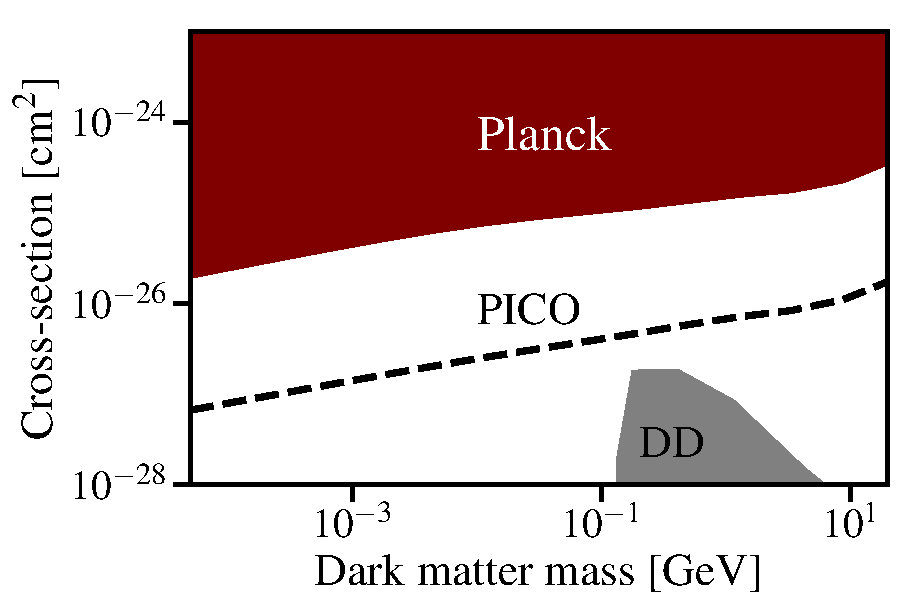
\includegraphics[width=0.50\textwidth]{images/pico_dd4.pdf}
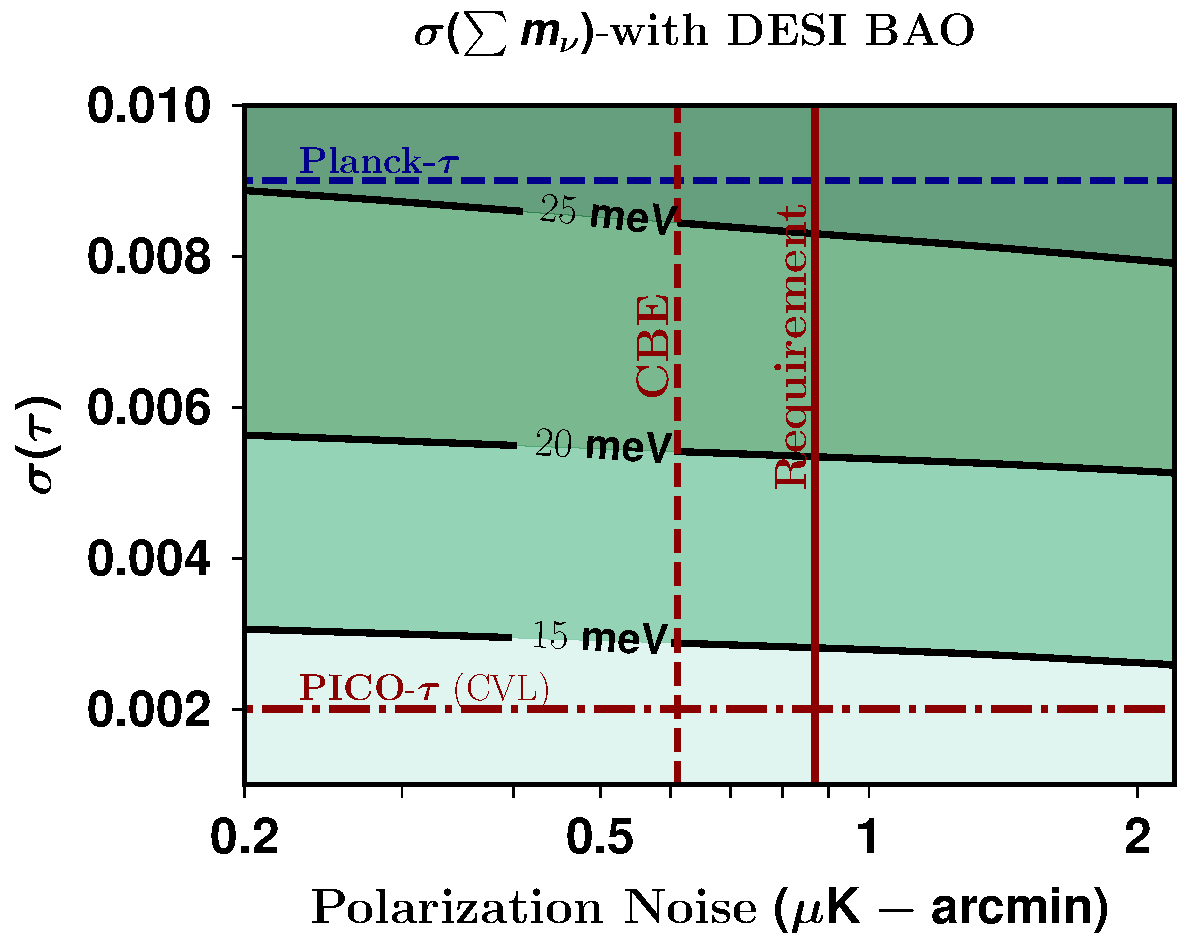
\includegraphics[width=0.48\textwidth]{images/Mnu_tauprior_final.pdf}
\vspace{-0.15in}
\caption{\captiontext {\bf Left:} PICO will give a factor of 25 more stringent constraint on the spin-independent velocity-independent dark matter scattering cross-section (dashed) relative to current \planck\ 95\% confidence limit (red)~\citep{2018PhRvL.121h1301G}. Terrestrial direct detection experiments are expected to give complementary and stronger constraints, but only for the higher dark matter masses (grey)~\cite{2018PhRvD..97l3013K}. 
{\bf Right:} Using a cosmic-variance-limited (CVL) measurement of $\tau,\, \sigma(\tau)=0.002$, \ac{BAO} information from DESI, and separation of foregrounds over 70\% of the sky, PICO will reach $\sigma(\Sigma m_{\nu}) = 14$~meV (contours), giving at least a $4\sigma$ detection of the minimal expected sum of neutrino masses $\Sigma m_{\nu} = 58$~meV. 
\label{fig:DM_baryons} }
\end{center}
\vspace{-0.2in}
\end{figure}
%

The axion is another dark matter candidate that is well motivated by string theory~\citep{Arvanitaki_etal} and that is consistent with straightforward extensions of the Standard Model of particle physics~\citep{peccei,weinberg,wilczek}. For an axion mass in the intermediate range $10^{-30} < m_a< 10^{-26} $~eV, current measurements constrain its fraction to be $\le 2$\% $(1\sigma)$ of the total dark-matter density. If 2\% of the total dark content is made of axions, PICO's measurement of the $TT$, $TE$ and $EE$ spectra with additional constraints from the lensing reconstruction will detect this species at between $7$ and $13\sigma$, depending on the mass range. %, as shown in Figure~\ref{fig:axions}. 
This is an average improvement of a factor of 10 relative to \planck .
% and a factor of two relative to the combination of \planck\ and S3, respectively, profoundly shaping our understanding of the nature of dark matter and its small-scale clustering. 

\noindent$\bullet$ {\bf Neutrino Mass} \hspace{0.1in} \label{neutrino_fundamental} The origin and structure of the neutrino masses is one of the great outstanding  questions about the nature of the Standard Model particles.  
%Measurements of neutrinos in the lab have revealed much  about the mass differences and mixing angles.  
Cosmology offers a  measurement of the sum of the neutrino masses $\sum m_\nu$ through the gravitational influence of the non-relativistic  cosmic neutrinos.  The current measurement of $\Neff = 2.99 \pm 0.17$~\citep{Planck2018_VI} already confirms the existence of these neutrinos at $>10\sigma$ and their mass implies that they will contribute to the matter density at low redshifts.  The best current mass constraint arises from a combination of  \planck~and BOSS \ac{BAO} giving $\sum m_\nu < 0.12$ eV (95\%) \cite{Planck2018_VI}.

Cosmological measurements are primarily sensitive to the suppression of power on small scales after the neutrinos become non-relativistic, which can be measured via CMB lensing (\S~\ref{sec:gravitationallensing}), or weak lensing in galaxy surveys.  However, these measurements are limited by our knowledge of the amplitude of the primordial fluctuation power spectrum $A_s$ because they only constrain the combination $A_s e^{-2 \tau}$, where $\tau$ is the optical depth to reionization. Although many astrophysical surveys hope to detect $\sum m_\nu$, any detection of the minimum value expected from particle physics, $\sum m_\nu = 58$~meV, at more than $2 \sigma$, will require a better measurement of $\tau$.
% and thus do not provide a high-precision measurement of either $A_s$ or $\tau$ separately.  \comor{we mention 'galaxy survey', but don't complete the thread of thought. Do we mean to say that the galaxy survey will be limited by the same degeneracy?}

The strongest constraints on $\tau$ come from the $EE$ spectrum at $\ell < 10$, which requires measurements over the largest angular scales  and good separation of Galactic foreground sources of emission. The best current measurement with $\sigma({\tau}) = 0.007$ is from \planck~\cite{Planck2018_VI}. With this uncertainty in $\tau$ one is limited to  $\sigma(\sum m_\nu) \gtrsim 25$ meV, after including forthcoming \ac{BAO} information (Fig.~\ref{fig:DM_baryons}, right); no other survey or cosmological probe will improve this constraint, unless a more accurate measurement of $\tau$ is made. One of the S3 experiments is attempting to measure the lowest $\ell$s and improve upon the \planck\ precision by a factor of about two~\citep{class}. A space mission with its access to the entire sky and broad frequency coverage is the most suitable platform for the measurement~(\S~\ref{sec:signal_separation} and \S~\ref{sec:complementarity}). PICO will reach the cosmic-variance limit uncertainty on $\tau$, $\sigma(\tau) = 0.002$~(\S~\ref{sec:luminoussources}), and using its deep CMB lensing map (\S~\ref{sec:gravitationallensing}) will therefore reach $\sigma(\sum m_\nu) = 14$ meV when combined with measurements of \ac{BAO} from DESI or Euclid~\cite{Levi:2013gra}.
%(without \ac{BAO} data the constraint is $\sigma(\sum m_\nu) = 43$ meV).
This measurement will give a $4\sigma$ detection of the minimum sum (SO3). 

%Robustly detecting neutrino mass at  $> 3\sigma$ in any cosmological setting is only possible with an improved measurement of $\tau$, like the one achievable with PICO. This measurement will give $\sum m_\nu>0$ at greater than $4\sigma$ or would exclude the inverted hierarchy ($\sum m_\nu > 100$ meV) at 95\% confidence, depending on the central value of the measurement.  Lab-based measurement could determine the hierarchy before PICO, but only cosmology can measure $\sum m_\nu$.

%%%%%%%%%%%%%%%%%%%%%%%%%

\subsubsection{Fundamental Fields: Primordial Magnetic Fields and Cosmic Birefringence}

$\bullet$ {\bf Primordial Magnetic Fields} \hspace{0.1in} One of the long-standing puzzles in astrophysics is the origin of observed 1--10~$\mu$G galactic magnetic fields~\citep{Widrow:2002ud}. Producing such fields through a dynamo mechanism requires a primordial seed field~\citep{Widrow:2011hs}. Moreover, $\mu$G-strength fields have been observed in proto-galaxies that are too young to have gone through the number of revolutions necessary for the dynamo to work~\citep{Athreya:1998}. A primordial magnetic field (PMF), present at the time of galaxy formation, could provide the seed or even eliminate the need for the dynamo altogether. Specifically, a 0.1~nG field in the intergalactic plasma would be adiabatically compressed in the collapse to form a $\sim$1~$\mu$G galactic field~\citep{Grasso:2000wj}.
PMFs could have been generated in the aftermath of phase transitions in the early Universe~\citep{Vachaspati:1991nm}, during inflation~\cite{Turner:1987bw,Ratra:1991bn}, or at the end of inflation~\cite{DiazGil:2007dy}. A detection of PMFs with the CMB would be a major discovery because it would establish the magnetic field's primordial origin, signal new physics beyond standard models of particle physics and cosmology, and discriminate among different theories of the early Universe~\cite{Barnaby:2012tk,Long:2013tha,Durrer:2013pga}.

The current CMB bounds on PMF strength are $B_{\rm 1\,Mpc}<1.2$ nG at 95\% CL for the scale-invariant~PMF spectrum \cite{Planck2015PMF,Kunze2015,Chluba2015PMF,Zucca:2016iur}, based on measurements of the $TT$, $TE$, $EE$, and $BB$ spectra.\footnote{It is conventional to quote limits on the PMF strength smoothed over a $1$~Mpc region in comoving units,  i.e., rescaled to $z=0$: $\mathbf{B}_{\rm today} = a^2\mathbf{B}(a)$.} 
%In particular, PMF sourced vector modes contribute to the $BB$ power spectrum at high $\ell$ \cite{Lewis:2004ef}. 
The much more accurate measurement of $BB$ by PICO would only marginally improve the PMF bound because CMB spectra scale as $B^4_{\rm 1\,Mpc}$. However, Faraday rotation provides a signature that scales linearly with the strength of PMFs~\cite{Kosowsky:1996yc}. It converts CMB $E$ modes into $B$ modes, generating mode-coupling $EB$ and $TB$ correlations. So far this signature has been out of reach because prior experiments did not have sufficient sensitivity. Using Faraday rotation, PICO will probe PMFs as weak as 0.1~nG ($1\sigma$), a precision that already includes the effects of imperfect lensing subtraction, Galactic foregrounds~\cite{Oppermann:2011td,De:2013dra,Pogosian:2013dya}, and other systematic effects. With this precision, which is a factor of five stronger than achievable with S3 experiments, PICO can conclusively rule out the purely primordial (i.e., no-dynamo driven) origin of the largest galactic magnetic fields. \\
%
$\bullet$ {\bf Cosmic Birefringence} \hspace{0.1in}
A number of well-motivated extensions of the Standard Model involve (nearly) massless axion-like pseudo-scalar fields coupled to photons via the Chern-Simons interaction term~\citep{Freese:1990rb,Frieman:1995pm,Carroll:1998zi,Kaloper:2005aj}. These couplings also generically arise within quintessence models for dark energy~\citep{Carroll:1998zi}, chiral-gravity models~\citep{2008PhRvL.101n1101C}, and models that produce parity-violation during inflation~\cite{Gluscevic:2010vv}. Regardless of the source of the parity-violating coupling, its presence may cause cosmic birefringence -- a rotation of the polarization of an electromagnetic wave as it propagates across cosmological distances~\cite{Harari:1992ea,Carroll:1989vb,Carroll:1998zi}. Cosmic birefringence converts primordial $E$-modes into $B$-modes, producing $TB$ and $EB$ cross-correlations whose magnitude depends on the statistical properties of the rotation field in the sky~\cite{Kamionkowski:2008fp,Gluscevic:2009mm,Gluscevic:2012me}. Previous studies have constrained both a uniform rotation angle as well as anisotropic rotation described by a power spectrum \cite{Gluscevic:2012me}. The current bound on a uniform angle is 30\arcmin\ (68\%)~\cite{Planck2016_XLIX}, and the bound on the amplitude of a scale-invariant rotation angle spectrum, which could be caused by fluctuations in a light pseudo-scalar field present during inflation~\cite{Pospelov:2008gg}, is 0.11~deg$^2$ (95\%)~\citep{Array:2017rlf}). Using the combination of five bands in the 70--156~GHz range, PICO will reduce the 95\% CL bound on the uniform rotation angle by a factor of 300, to 0.1\arcmin.  
%, assuming that the beam can be calibrated to reach the main science goals without \emph{assuming} vanishing parity-odd spectra of $EB$ and $TB$ type. 
The 95\% CL bound on the amplitude of a scale-invariant rotation spectrum will be reduced by a factor of 275 to $4\times10^{-4}$~deg$^2$, giving important constraints on string-theory-motivated axions~\cite{Svrcek:2006yi,Pospelov:2008gg}.


%The simplest model for late-time acceleration of the Universe is with a slowly-evolving scalar field, also called quintessence~\cite{Carroll:1998zi}. Such a field generically couples to electromagnetism through a Chern Simons-like term, and causes linear polarization of photons propagating cosmological distances to rotate. This is known as cosmic birefringence~\cite{Carroll:1998zi}. The birefringence converts primordial $E$-modes into $B$-modes. It thus produces parity-violating $TB$ and $EB$ cross-correlations whose magnitude depends on the statistical properties of the rotation field in the sky~\cite{Kamionkowski:2008fp,Gluscevic:2009mm}. There are no theoretical predictions for the level of birefringence, but if observed, it would be evidence for physics beyond the standard model and a potential probe of dark-energy microphysics~\citep{Gluscevic:2009mm,Caldwell:2011,yadav2009}. 


\end{document}

